%%% LaTeX Template: Article/Thesis/etc. with colored headings and special fonts
%%%
%%% Source: http://www.howtotex.com/
%%% Feel free to distribute this template, but please keep to referral to http://www.howtotex.com/ here.
%%% February 2011
%%%
%%% Last updated September 2021 by CDM

%%%  Preamble
\documentclass[11pt,letterpaper]{article}
\usepackage[margin=1.0in]{geometry}
\usepackage[T1]{fontenc}
\usepackage[bitstream-charter]{mathdesign}
\usepackage[latin1]{inputenc}					
\usepackage{amsmath}						
\usepackage{xcolor}
\usepackage{cite}
\usepackage{hyphenat}
\usepackage{graphicx}
\usepackage{float}
\usepackage{subfigure}
\usepackage{sectsty}
\usepackage[compact]{titlesec} 
\usepackage[tablegrid]{vhistory}
\allsectionsfont{\color{accentcolor}\scshape\selectfont}

%%% Definitions
\definecolor{accentcolor}{rgb}{0.0,0.0,0.5} 
\newcommand{\teamname}{Robo Crew}
\newcommand{\productname}{RV8 Robot Work Cell}
\newcommand{\coursename}{CSE 4316: Senior Design I}
\newcommand{\semester}{Fall 2023}
\newcommand{\docname}{Project Charter}
\newcommand{\department}{Department of Computer Science \& Engineering}
\newcommand{\university}{The University of Texas at Arlington}
\newcommand{\authors}{Akshay Paluri \\ Ameen Mahouch \\ Muhammad Anas \\ Kundan Singh Mahato \\ Hyun Ho Kim}

%%% Headers and footers
\usepackage{fancyhdr}
	\pagestyle{fancy}						% Enabling the custom headers/footers
\usepackage{lastpage}	
	% Header (empty)
	\lhead{}
	\chead{}
	\rhead{}
	% Footer
	\lfoot{\footnotesize \teamname \ - \semester}
	\cfoot{}
	\rfoot{\footnotesize page \thepage\ of \pageref{LastPage}}	% "Page 1 of 2"
	\renewcommand{\headrulewidth}{0.0pt}
	\renewcommand{\footrulewidth}{0.4pt}

%%% Change the abstract environment
\usepackage[runin]{abstract}			% runin option for a run-in title
%\setlength\absleftindent{30pt}			% left margin
%\setlength\absrightindent{30pt}		% right margin
\abslabeldelim{\quad}	
\setlength{\abstitleskip}{-10pt}
\renewcommand{\abstractname}{}
\renewcommand{\abstracttextfont}{\color{accentcolor} \small \slshape}	% slanted text

%%% Start of the document
\begin{document}

%%% Cover sheet
{\centering \huge \color{accentcolor} \sc \textbf{\department \\ \university} \par}
\vspace{1 in}
{\centering \huge \color{accentcolor} \sc \textbf{\docname \\ \coursename \\ \semester} \par}
\vspace{0.5 in}
\begin{figure}[h!]
	\centering
   	
\includegraphics[width=0.60\textwidth]{images/robocrew.jpg}
\end{figure}
\vspace{0.5 in}
{\centering \huge \color{accentcolor} \sc \textbf{\teamname \\ \productname} \par}
\vspace{0.5 in}
{\centering \large \sc \textbf{\authors} \par}
\newpage


%\vspace{1 in}
%\centerline{January 13th, 2012}
%\newpage

%%% Revision History
\begin{versionhistory}
  	\vhEntry{0.1}{09.24.2023}{AP, AM, HK, KM, MA}{Document creation}
\end{versionhistory}
\newpage

%%% Table of contents
\tableofcontents
\newpage

%%% List of figures and tables (optional)
\listoffigures
%\listoftables
\newpage
\setcounter{table}{0}

%%% Executive summary sections
\section{Problem Statement}
In the realm of advancing robot arm technology, we must confront several critical challenges. Safety is of paramount concern as robot arms need to collaborate closely with human workers during various tasks. Ensuring the well-being of personnel while harnessing the advantages of robot arms necessitates the implementation of safety control systems and sensors.

Additionally, there is the challenge of societal acceptance. Achieving recognition and acceptance of robot arms in society is crucial. To accomplish this, we must focus on promoting and enhancing education about robot arm technology, ensuring that the public comprehends the benefits and potential of these machines.

As technological advancement accelerates, devices equipped with new technologies continue to emerge. Consequently, factors such as product weight, completeness, and precision have gained increasing importance. Addressing these challenges entails reducing component sizes, adopting more intricate designs, and mitigating the potential risks of errors in sensitive operations, particularly those involving human life. Tasks demanding delicate manipulation may surpass the limits of human physical capabilities. Hence, it is imperative that we work diligently to overcome these challenges.
\section{Methodology}
In this project, we improve and teach Mitsubishi Electric Industrial Robot, RV8, to execute specific tasks. Safety enhancements include the integration of new lighting systems and emergency stop mechanisms for operator protection. The RV8's 8 controllable joints, accessible via the Robot Teaching Box, enable precise control, with the robot capable of autonomous learning, manual movement execution, and object manipulation via a vision sensor. Various algorithms are integrated to enhance task efficiency. Future plans involve attaching an end-effector for object manipulation. Through this methodology, we aim to harness the RV8's capabilities while ensuring safety and efficiency in a range of tasks, with an eye toward future developments.
\section{Value Proposition}
In today's rapidly evolving technological landscape and increasingly industrialized world, robot arms are emerging as versatile and essential tools. These sophisticated machines are set to revolutionize industries through several promising trends in development.
Firstly, there is the exciting frontier of enhanced intelligence, where artificial intelligence and machine learning empower robot arms to learn autonomously and make decisions. Equipped with advanced sensors and vision systems, these robot arms gain heightened environmental awareness and object recognition, making them more adaptable to dynamic scenarios. Additionally, the growing need for collaboration with humans requires robot arms to perceive human movements and intentions, ensuring secure and seamless cooperation. In parallel, advancements in unmanned technology allow robot arms to operate autonomously in specialized environments such as hazardous settings, space exploration, and deep-sea exploration. This autonomy improves task safety and efficiency and expands the range of operations. Finally, there is a focus on integration, facilitated by modular and standardized designs, which simplifies complexity and enables quick configuration for diverse tasks. In summary, these trends position robot arms as essential catalysts for increased productivity, efficiency, and safety across various industries. They will tackle complex challenges and unlock remarkable outcomes for the future.
\section{Development Milestones}
The following is a list of completion dates for all major documents, demonstrations, and associated deadlines:
\begin{itemize}
  \item Project Charter first draft - September 25, 2024
  \item System Requirements Specification - October 16, 2024
  \item Architectural Design Specification - November 6, 2024
  \item Detailed Design Specification - February 12, 2024
  \item Demonstration of Initial Robot Movement - September 25, 2024
  \item Demonstration of Basic Program - October 16, 2024
  \item Demonstration of Linear Rail Movement - November 6, 2024
  \item Demonstration of E-stop Switch Configuration - November 06, 2024
  \item Demonstration of holder for paint brush - February 12, 2024
  \item Demonstration of GPIO 20-Pins Configuration - March 7, 2024
  \item Demonstration of Light Tower Setup - March 25, 2024
  \item Demonstration of Spray oil paint Program - April 15, 2024
  \item CoE Innovation Day poster presentation - April 16, 2024
  \item Final Project Demonstration - April 26, 2024
  \item Final Project Submission - May 08, 2024
\end{itemize}
\newpage

%%% Remaining project charter sections
\section{Background}
In the rapidly evolving landscape of warehousing and logistics, the conventional approach to material handling in warehouses contains several challenges. Palletizing and depalletizing boxes manually is a time-consuming task, which decreases productivity. Consequently, labor costs associated with manual palletizing and depalletizing are increased, encompassing wages, benefits, and additional expenditures associated with managing a workforce engaged in repetitive physical activities. Moreover, manual material handling poses inherent risks to the workforce. Accidents and injuries are a constant concern, impacting both employee well-being and company reputation. The physically demanding nature of tasks can also lead to reduced job satisfaction. Finally, with modern commerce continuing to grow, warehouses must adapt to higher volumes of goods and fulfill needs with efficiency. Manual processes often hinder the ability to meet customer demands effectively.

The integration of robotic arms for palletizing and depalletizing tasks is no longer a matter of convenience, but a necessity. The shift towards automation is driven by the pitfalls of manual labor listed above, as well as several compelling factors consistent in robotic arms that demonstrate its ability to address these challenges effectively and revolutionize material handling in warehouses. Robotic arms excel at repetitive tasks requiring precision. The consistency of robot arms translates to significant improvements in efficiency, ultimately allowing faster order fulfillment and throughput rates. Robotic arms are also largely scalable. With a large rise in e-commerce, robotic arms can adapt to seasonal demand, and can shift workload to accommodate responsively in a dynamic marketplace. In addition to their agility in a demanding environment, robotic arms provide product integrity. In industries like food and pharmaceuticals, robotic arms are programmed to handle goods aligning with quality standards issued by the Occupational Safety and Health Administration (OSHA). This not only guarantees product integrity, but also compliance with industry-specific regulations.

The University of Texas at Arlington has a Mitsubishi Electric RV-8CRL Robot housed in room 335 of the Engineering Research Building. Previous teams of students and Dr. Christopher McMurrough have worked on the hardware setup of the work cell, including the MELSEC Programmable Logic Controller (PLC). The RV-8 also is mounted to a linear rail, enabling its 7th axis. While the robot is operational, the work cell still needs several areas of integration completed. The laser safety scanners create virtual safety zones around the robot, monitoring the surrounding area for any human intrusion. These laser scanners are not implemented yet. There are two emergency stop (E-stop) switches in and around the work cell, providing immediate and highly visible means to shut down the robot in the case of an emergency. Currently, the emergency stops are functional but wired inefficiently. The linear rail was most recently installed with aims to enhance reach and flexibility of the robot. At present, the linear rail is not integrated with the RV-8 robot and is not functional.

The sponsor of this project, Dr. McMurrough, aims for this project to finish the integration of the work cell, with the hopes that it serves as an invaluable resource for both research and educational purposes at UTA. The robot is within a glass encasing shown to onlookers in the building. Thus, this project hopes to showcase the functionalities of the robot to a wider audience and spark interest at the consistent innovation within Computer Science and Engineering at UTA. The completed work cell will empower students with hands-on experience, allowing them to explore the frontiers of robotics, automation, and control systems. 

\section{Related Work}

Factory automation, including robotic painting systems, is emerging as a state-of-the-art technology in manufacturing. There are several current implementations of robotics that address the current challenges in factory automation. Several companies offer robotic systems designed specifically for painting applications. A pioneer in these types of robots is ABB's Delta line of robots, most notably the FlexPicker IRB 360 \cite{robotsdonerightHistoryRobots}. The first prototype was designed by a research group led by Professor Reymond Clavel at EPFL, Switzerland \cite{bonev_delta_2001}. The groundbreaking robot was based on the concept of parallelograms, where three parallelograms restricted the mobile platform's orientation to three purely translational degrees of freedom. The robot's actuation involves rotating levers with revolute joints, which can be actuated using rotational motors or linear actuators. Its lightweight construction and base-mounted actuators make it ideal for light objects between 10 grams to 1 kilogram \cite{bonev_delta_2001}. Covered by over 30 patents, the robot's success is seen in several industries including automotive manufacturing, electronics, and aerospace.

Another notable robotic system in factory automation from ABB's product line is the IRB 6700 Series. Similar to the RV-8CRL, an IRB 6700 robot is a vertical robotic solution with six degrees of freedom. The series has an impressive payload range between 150 to 300 kilograms, with a max reach of 3.2 meters \cite{robotics2021product}. The line even includes variants available as floor mounted and inverted versions, matching the orientation of UTA's RV-8CRL. Other series designed by ABB include the IRB 2600 line, IRB 140 line, and YuMi robots.

FANUC's M-20 series of robots represent a versatile solution for medium payload painting tasks in manufacturing. This line of robots have a payload capacity of 35 kilograms and a max reach of 1,811 millimeters \cite{connolly2007new}. The robot is strong, yet reasonably light. The 6-axis machine's design incorporates a hollow upper arm, and is ideal for multi-material handling. Its compact footprint allows it to work efficiently in confined spaces, optimizing space utilization within the factory. FANUC's dedication to reliability is reflected in the M-20 series, as it boasts an industry leader long Mean Time Between Failures (MTBF) figure, up to 11 years \cite{aggogeri2020robotic}. Other series designed by FANUC include the CR series and R-30iB series.

KUKA, a German robotics company, offers a range of robots suited for painting and automation tasks in manufacturing. Their KR AGILUS series, for example, provides high-speed and precise handling capabilities for small and medium payloads \cite{muftooh20186}. On the other hand, Yaskawa Motoman, a subsidiary of Yaskawa Electric Corporation, specializes in industrial robots for various applications, including painting in manufacturing. The Motoman MH series offers versatility and efficiency in painting tasks \cite{muftooh20186}. Additionally, companies like Universal Robots and MiR (Mobile Industrial Robots) have gained prominence for their collaborative and autonomous mobile robots that can work alongside human workers in factory environments.

As robots are becoming more technologically available, manufacturing industries are adopting the technology with frequency. According to ABI Research, a global tech market advisory firm, worldwide commercial robot revenue in factories will have a Compounded Annual Growth Rate (CAGR) of over 23% from 2021 to 2030 and exceed $51 billion by 2030 \cite{nytimesRobotsArent}. This is seen with industry leaders like automotive manufacturers, who are increasingly investing in robotic painting systems within their production facilities.

Locally, companies are building factories with an aim at reducing human labor. Companies like Tesla have been researching with their robotic painting systems, which have capabilities of painting and coating various automotive parts. Operating at a facility in Dallas, Texas, these systems are capable of handling a significant portion of the painting process \cite{dallasnewsBattleHumans}. As these companies continue to innovate and invest in automation solutions, the manufacturing industry is poised for a transformative shift marked by increased efficiency, reduced operational costs, and improved product quality.
\section{System Overview}
This section defines the top-level logical view of the design and describes the detail architectural strategy for the RV8 work cell system flow. Three separate layers make up the structure of the system: input, processing, and output. With the help of these layers, which are all essential to the system, the robot is able to carry out dynamic tasks that are dependent on the processing of sensor data. A high-level block diagram that shows the connections and interactions between different layers is included in this part to provide readers a thorough understanding of the architecture of the entire system. A robotic system's input layer, which makes use of sensors like a gate sensor and an E-stop is essential for task execution. E-stops offer an emergency shutdown signal that allows the system to be stopped right away. The robot arm's speed is controlled by the Gate sensor, which also communicates with the controller to find out the cage gate's present state. Efficiency and safety are prioritized in this design, which allows the robot to respond and adapt to a variety of scenarios while integrating security features like gate status monitoring and emergency stops. With the integration of sensors will perform the operation such as splashing multi-color paint to the desire target with great level of precision. PC and the trigger switch will be inter-connected to the PC to perform the necessary communication to perform the given task.  

\begin{figure}[h!]
	\centering
 	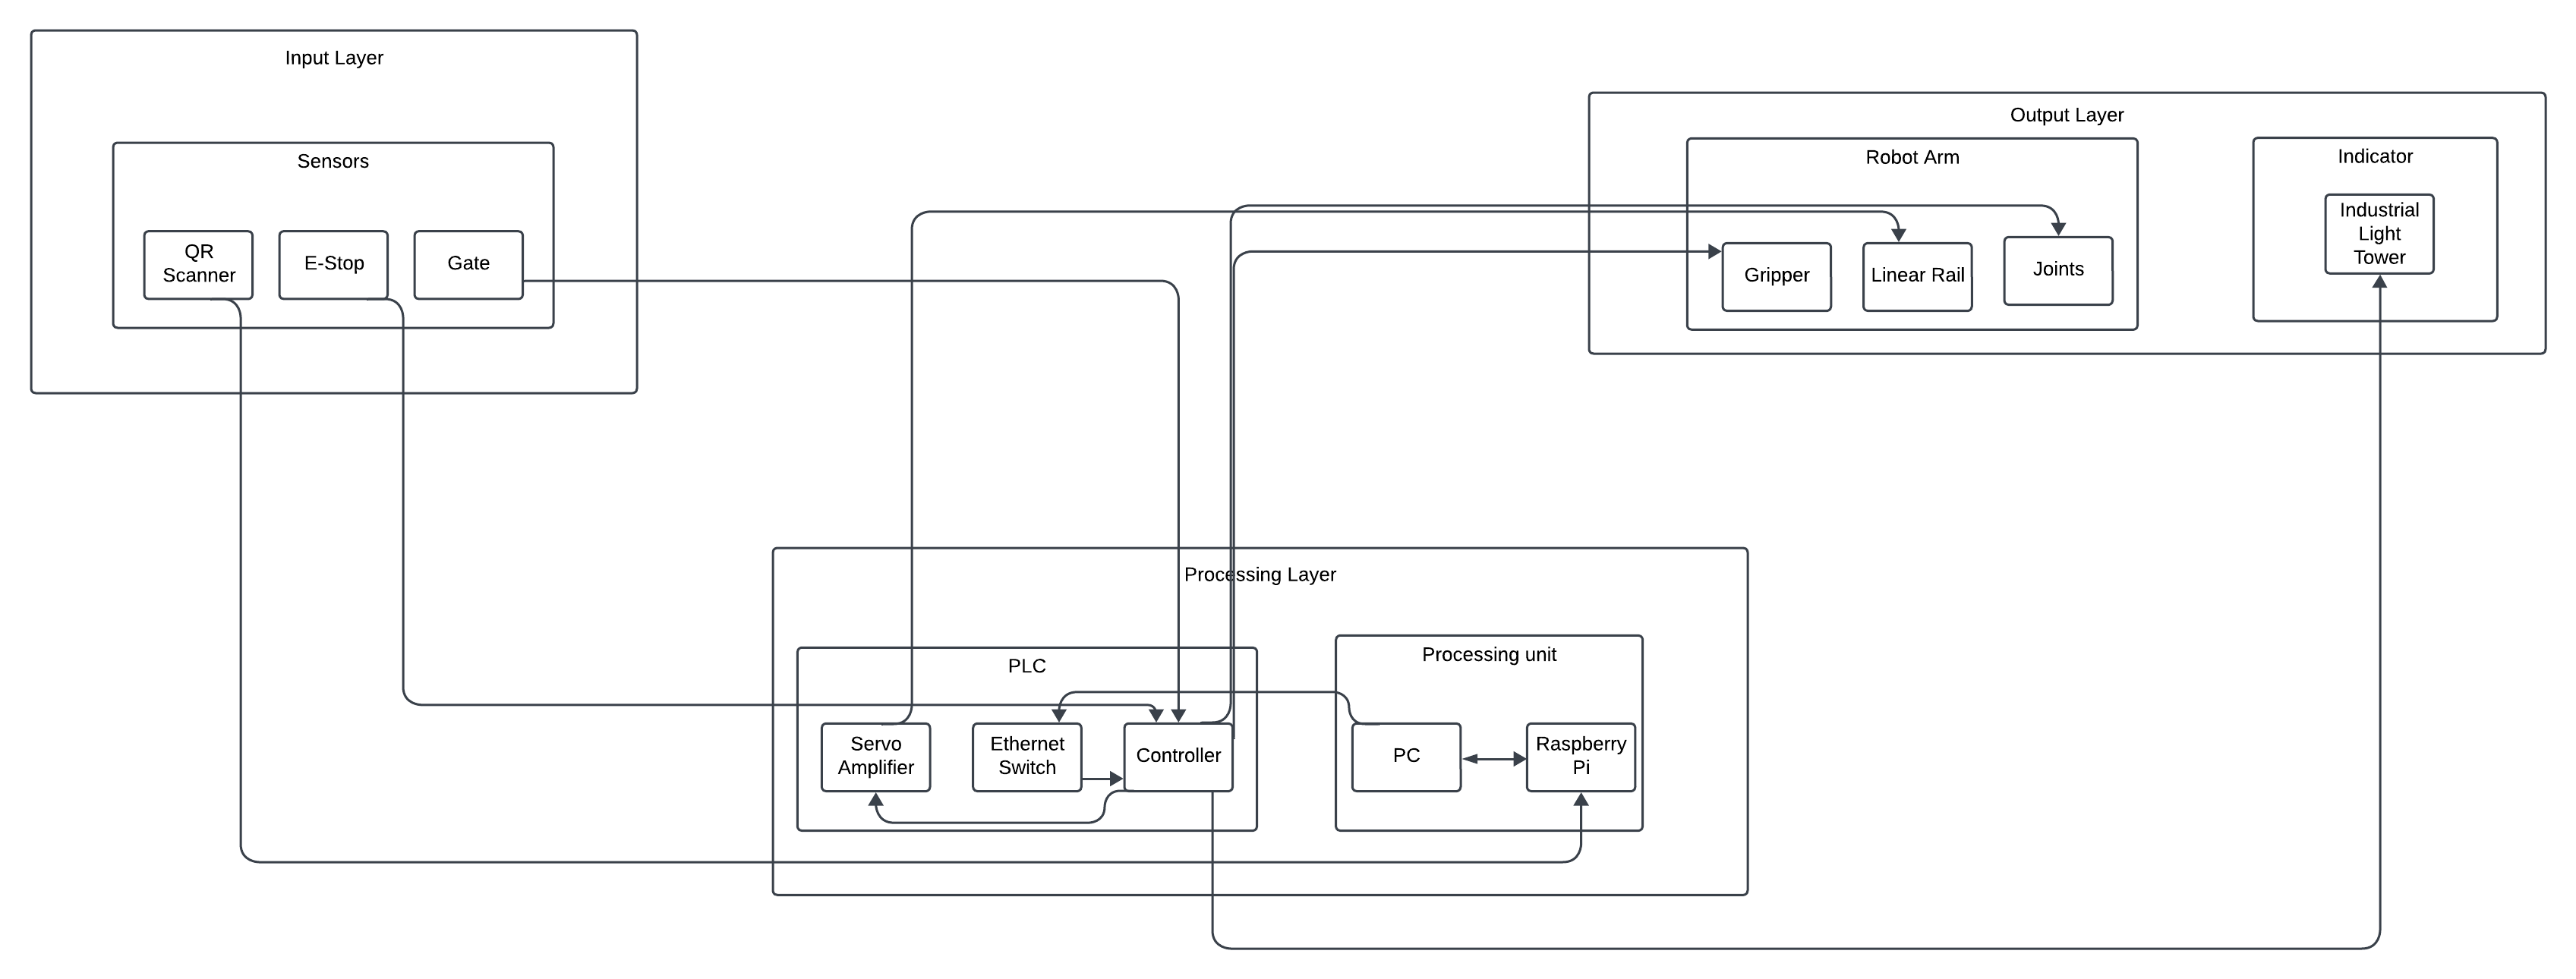
\includegraphics[width=1\textwidth]{images/system_subystem.png}
 \caption{System architecture}
\end{figure}

\section{Roles \& Responsibilities}
Our key stakeholder is Dr. Christopher McMurrough, the project sponsor and the designated point of contact from the sponsor side. Mitsubishi RV-8CRL Robot and essential project materials will be provided by the project sponsor, facilitating the project's implementation. The project team includes five undergraduate students from the Computer Science and Engineering (CSE) department at the University of Texas at Arlington (UTA). The software engineer on the team is Ameen Mahouch. Additionally, there are three team members with a background in Computer Science: Akshay Paluri, Muhammad Anas, and Hyun Ho Kim. With a Computer Engineering background, Kundan Singh Mahato is also part of the team. The workload within the group will be distributed equally among all team associates to provide efficient improvement and successful task fulfillment. The team will decide that each team member will have reasonable support in responsibilities and duties.
\section{Cost Proposal}
The project aims to program the robot for precise and accurate painting. To create a fully functional system, we require additional components. These include an air compressor and an airbrush, which must be attached to the robot. Additionally, inductive sensors are necessary to enable the robot to operate on the additional linear rail axis.

%The project focuses on programming the Mitsubishi RV-8CRL robot for efficient box pelletizing in a warehouse setting, and several major expenses are expected. The investment of a software license for programming the robot is required, ensuring that the RV-8CRL's capabilities are fully utilized and seamlessly melded into the preferred pelletization process and investment in a Mitsubishi Gripper, tailored to the specifications and requirements of the RV-8CRL robot, is essential to enable the precise handling of boxes during the pelletization task. Functional units necessary for the robot's seamless operation, including sensors for safety and coordination and any customized fixtures to optimize the pelletizing process, are crucial components of the project's expenditure. 

\subsection{Preliminary Budget}

For the project's future development, several additional components are being considered to enhance the capabilities and efficiency of the Mitsubishi RV-8CRL robot in its paint spraying application the will be added in future documents.

\begin{table}[h]
    \centering
    \begin{tabular}{|c|c|} \hline 
         Items& Price\\ \hline 
         Air compressor with airbrush& 120\\ \hline
    \end{tabular}
\end{table}


\subsection{Current \& Pending Support}

\$800, the default funding given to  the Senior Design Project by CSE department.
\section{Facilities \& Equipment}
The RV8 Robot Work Cell project will be situated in ERB 335, a designated laboratory area. This lab area will include the electrical infrastructure to accommodate the power requirements of the RV8 robot, MELSEC, and PLC controllers. Safety measures are of paramount importance, and as such, emergency stop systems, safety barriers, and warning signs have been implemented and will be modified to create a secure working environment for both operators and equipment. Additionally, the layout of workstations within ERB 335 will be configured to optimize workflow efficiency, allowing operators to interact with the RV8 robot and associated equipment.

In terms of equipment, the RV8 Robot Work Cell will feature essential components. The RV8 robot itself will be the central robotic arm, equipped with advanced technology to provide precision, speed, and versatility in performing a wide range of tasks. The project will also incorporate a Mitsubishi Electric MELSEC controller as the central control unit, facilitating  coordination and synchronization of the robot's actions. Programmable Logic Controllers (PLCs) will be  positioned to manage auxiliary equipment and processes within the work cell Furthermore, to complement the RV8 robot's capabilities, a gripper will be outsourced from a reputable supplier, selected based on its compatibility and suitability for handling various materials and objects within the work cell. Additionally, the work cell will incorporate a linear rail with a motor attached to it, a key feature for controlled and precise linear movement of the RV8 robot. This motor will be  connected to the PLC controller, allowing for precise control over the linear motion of the robot along the rail. The linear rail will be provided in the laboratory as well and will require reading of several manuals from Mitsubishi to configure the movement of the linear rail.

\section{Assumptions}
\begin{itemize}
  \item ERB 335 will provide all equipment needed to program the movement for the robot arm
  \item The Engineering Research Building will provide for reliable internet connection and ample power connectivity
  \item Security measures such as emergency stop will work as intended and will stop the movement of robot arm once pressed
  \item Once the air brush arrives, it will work as intended and will meet the quality standard needed with the robot arm
  \item The development team will be notified of any problems that may occur in the Engineering Research Building (ERB)
\end{itemize}

\section{Constraints}
\begin{itemize}
  \item Final prototype demonstration must be completed by the beginning of Q2, 2024
  \item The programming and movement shall only happen in ERB 335a.
  \item LOTO or Lockout Tagout procedure must be used to prevent unauthorized personnel to access the robot arm.
  \item Total development costs must not exceed \$800.
  \item The robot arm should only be programmed via the host PC and any wiring shall be connected via the PLC.
\end{itemize}

\section{Risks}
\begin{table}[H]
\resizebox{\textwidth}{!}{
\begin{tabular}{|l|l|l|l|}
\hline
 \textbf{Risk description} & \textbf{Probability} & \textbf{Loss (days)} & \textbf{Exposure (days)} \\ \hline
 Availability of air brush due to poor 3D printing  & 0.80 & 5 & 4 \\ \hline
 Air brush, along with robot arm could damage its environment & 0.30 & 15 & 4.5 \\ \hline
 Internet delays that may cause delay in the program of the robot arm  & 0.30 & 9 & 2.7 \\ \hline
 Mishandling of electrical components and/or the PLC  & 0.05 & 30 & 1.5 \\ \hline
 Poor integration of the air brush with robotic arm and linear rail & 0.30 & 10 & 3 \\ \hline
\end{tabular}}
\caption{Overview of highest exposure project risks}
\end{table}

\section{Documentation \& Reporting}
%%% In this section, you will describe all of the various artifacts that you will generate and maintain during the project life cycle. Describe the purpose of each item below, how the content will be generated, where it will be stored, how often it will be updated, etc. Replace the default text for each section with your own description. Reword this paragraph as appropriate.

\subsection{Major Documentation Deliverables}
The major documentation deliverables for this project are project charter, System requirement specification, detailed design specification. Sprint 1 will cover project charter document. The duration for each sprint in this project is 2-weeks long (default length for any new team when assigned the project). The first half of the project is consisting of total number of 4 sprints. First sprint will deliver the project charter. System requirement specification will be delivered the second sprint. Third and fourth sprint will consist of Architectural design specification and detailed design specification including Phase I demo. 

\subsubsection{Project Charter}
This document will be completed by the end of first sprint. Although this document will be altered and updated as required. Since the team has not started working on this project physically things might be added or updated or removed.  


\subsubsection{System Requirements Specification}
This document is planned for sprint two. The requirements specifications will be written by the end of second sprint. Since following the agile methodology this document will be modified as required for certain specifications. This will be delivered by the end of sprint 3 (October 16, 2023). 

\subsubsection{Architectural Design Specification}
Architectural Design will be initiated in sprint 3. This will be maintained and modified as per the change in requirement or plan. This will be delivered by the end of sprint 3 (November 6, 2023). 

\subsubsection{Detailed Design Specification}
Detailed design specifications will also be delivered by the end sprint 3. The document would be altered if the team finds a necessary change. 

\subsection{Recurring Sprint Items}


\subsubsection{Product Backlog}
Items will be added to backlog based on SRS. These items will be prioritized by the complexity and necessity to reach the goal of the sprint and progress towards end result. Team will use excel to track the backlog. These backlogs will be discussed in meetings. 

\subsubsection{Sprint Planning}
Each sprint will be planned after the termination of previous sprint. There are going to be a total of 8 sprints (Senior Design I has 4 sprints and Senior Design II has 4). 

\subsubsection{Sprint Goal}
The team will decide collaboratively about the sprint goal.  

\subsubsection{Sprint Backlog}
The teams will determine which task or tasks will make it to backlog. 

\subsubsection{Task Breakdown}
Different tasks will be assigned to team members. The task can have a sub team of 2-3 members working on it or it can also be assigned to an individual team member depending upon the complexity of the task. 

\subsubsection{Sprint Burn Down Charts}
The team will decide the burn down charts. This will use MS-Excel. 

\begin{figure}[h!]
    \centering
    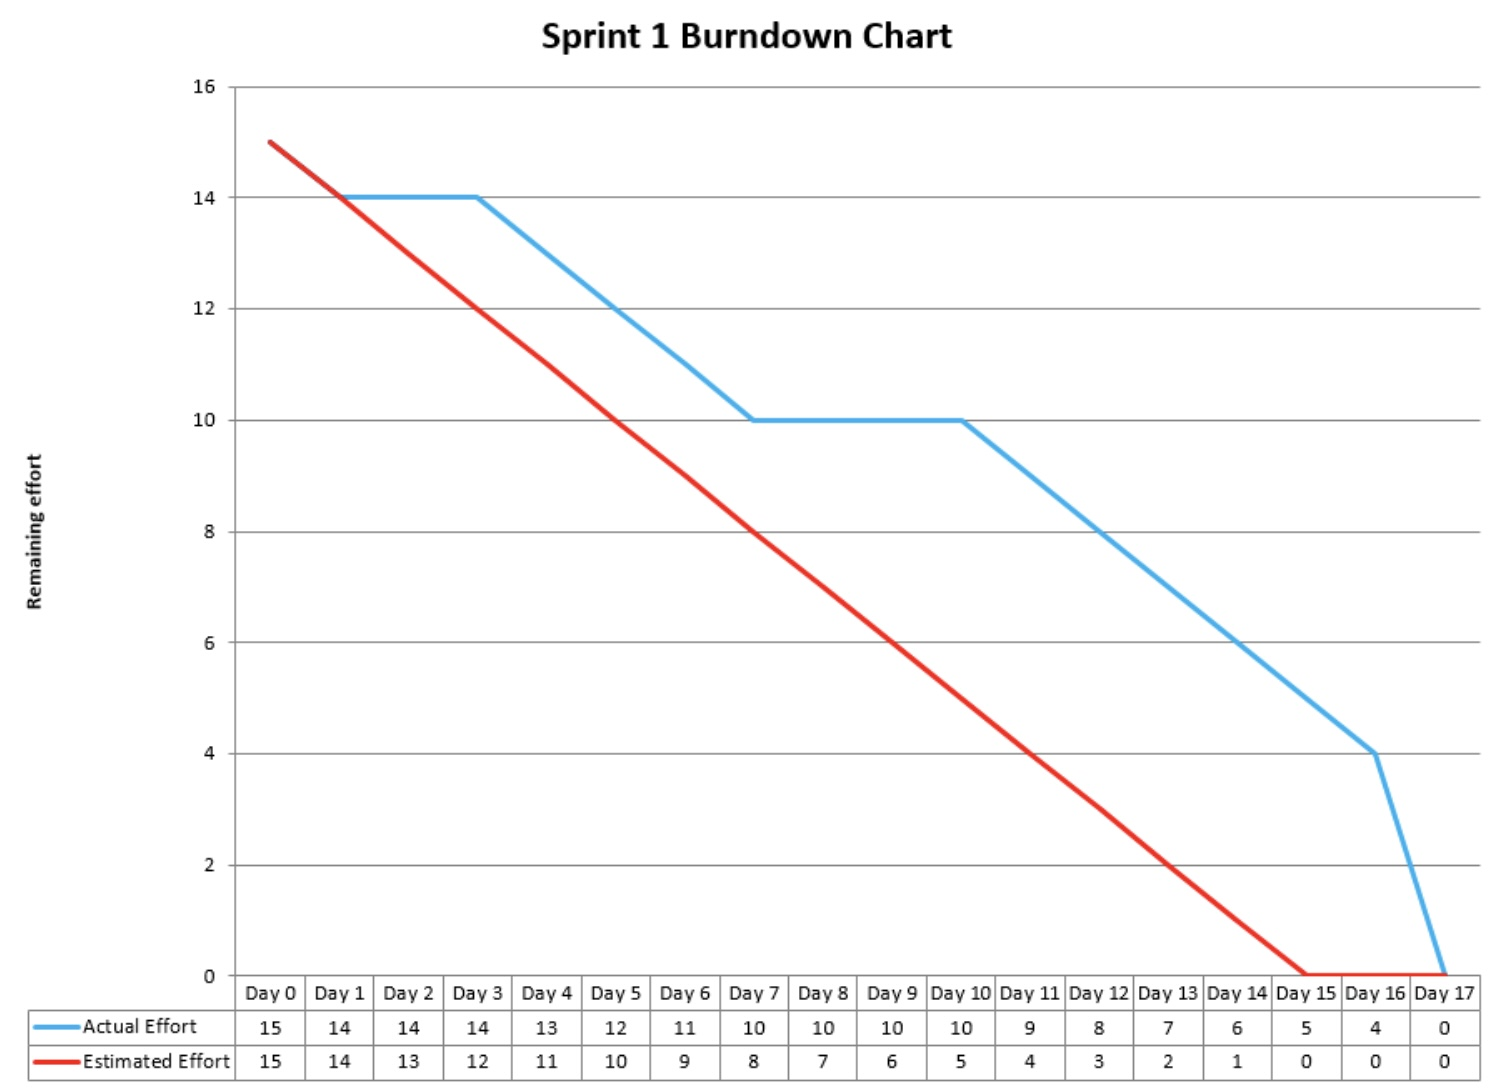
\includegraphics[width=0.5\textwidth]{images/burndown_example.jpg}
    \caption{Example sprint burn down chart}
\end{figure}

\subsubsection{Sprint Retrospective}
The retrospective will be handled after carrying out a conversation regarding the previous sprint. Individuals are required to report any sort issues and inconvenience before the sprint end so that important measure can be taken before the sprint ends. Lastly, next sprint goals and previous sprint\'s incompletion (if any) will be discussed before the start of new sprint.  

\subsubsection{Individual Status Reports}
An individual must report the progress that was being through the sprint which will also be recorded. Peer Review will ensure that the team is in the best possible way of communications and are good aware of the other members strengths and weaknesses regarding this project. 

\subsubsection{Engineering Notebooks}
Engineering notebooks will not be used. 

\subsection{Closeout Materials}

\subsubsection{System Prototype}
The final system prototype will include a working RV8 robot arm with a linear rail. This will be demonstrated through a video as well as in the lab where it is setup. 

\subsubsection{Project Poster}
The project poster will discuss the system overview of the project. The overview will include the design and architectural details. It will be delivered after the system prototype is ready. 

\subsubsection{Web Page}
The project webpage will be public and provide access to the documentation associated with the prototype such as project charter, SRS and ASD. This webpage will be updated throughout the project as the sprints will be put to finish. 

\subsubsection{Demo Video}
The demo video will be a source to display the use of the prototype and the purpose the prototype. 

\subsubsection{Source Code}
GitHub will be used as the repository to maintain and store code for this project. All the changes made will be pushed to GitHub. Using GitHub will give us the option to revert if any complication arises. Since the prototype is designed for specific purpose only, the code will be implemented. 

\subsubsection{Source Code Documentation}
The documentation will be provided in a PDF format. 

\subsubsection{Hardware Schematics}
This will be decided during ASD. 

\subsubsection{CAD files}
The prototype will contain a gripper. The team will try to obtain from external retailer. In case of unavailability of the part or if it is unsuited then the teams will use Inkscape to generate CAD files for the gripper and will use it to generate the gripper as designed. 

\subsubsection{Installation Scripts}
The customer will not be required to deploy any software as the team will deploy the software for them. There will be no updates in future for this project. Because this project is only required to fulfill certain task only. 

\subsubsection{User Manual}
The customer will be provided with a digital (PDF) and a printed manual for the project. 
\newpage

%%% References
\bibliographystyle{plain}
\bibliographystyle{reference/IEEEtran_custom}
\bibliography{reference/refs}{}

\end{document}